\documentclass[oneside]{scrbook}

\usepackage[utf8]{inputenc}
\usepackage[ngerman]{babel}
\usepackage{microtype}

\usepackage{scrhack} % Verschiedene Hacks für die Kompatibilität anderer Pakete mit KOMA-Script.

\usepackage{libertine}
\usepackage{amsmath,amssymb,amsthm}
\usepackage[libertine]{newtxmath} % Libertine Math.
\usepackage{commath}

\usepackage{wasysym}

\usepackage[T1]{fontenc}

% Schusterjungen und Hurenkinder
\widowpenalties 3 10000 10000 100
\clubpenalties 3 10000 10000 100
\displaywidowpenalty = 10000

\usepackage[german=guillemets]{csquotes}
\usepackage{booktabs}

\usepackage{xcolor}
\usepackage[pdftex]{graphicx}
\usepackage{tikz}
\usetikzlibrary{shapes}
\usepackage{hyperref}

\allowdisplaybreaks % Allows pagebreaking of aligned equations

\newtheoremstyle{myplain}% name
  {\topsep}% Space above
  {\topsep}% Space below
  {\itshape}% Body font
  {}% Indent amount
  {\bfseries\sffamily}% Theorem head font
  {}%Punctuation after theorem head
  {.5em}%Space after theorem head
  {}% theorem head spec

\newtheoremstyle{mydefinition}% name
  {\topsep}% Space above
  {\topsep}% Space below
  {\normalfont}% Body font
  {}% Indent amount
  {\bfseries\sffamily}% Theorem head font
  {}%Punctuation after theorem head
  {.5em}%Space after theorem head
  {}% theorem head spec

\newtheoremstyle{myremark}% name
  {\topsep}% Space above
  {\topsep}% Space below
  {\normalfont}% Body font
  {}% Indent amount
  {\itshape\sffamily}% Theorem head font
  {}%Punctuation after theorem head
  {.5em}%Space after theorem head
  {}% theorem head spec

\theoremstyle{myplain}
\newtheorem{proposition}{Satz}[chapter]

\theoremstyle{mydefinition}
\newtheorem{definition}[proposition]{Definition}
\newtheorem{example}[proposition]{Beispiel}
\newtheorem{remark}[proposition]{Bemerkung}

\newcommand{\N}{\mathbb{N}}
\newcommand{\R}{\mathbb{R}}
\newcommand{\Z}{\mathbb{Z}}
\newcommand{\C}{\mathbb{C}}
\newcommand{\T}{\mathbb{T}}

\DeclareMathOperator{\sinc}{sinc}

\newcommand{\TODO}[1]{{\color{red}\textbf{\textsf{TODO:}}~#1}}
\usepackage[pdftex]{graphicx}  
\usepackage{listings}

\newcommand{\INT}[1]{\text{d#1}}
\newcommand{\INTM}[1]{\text{d} #1}
\newcommand{\INTMM}[2]{\text{d#1}_{#2}}
\renewcommand{\T}[1]{\text{#1 }}
\newcommand{\DIFF}[2]{\frac{\INT{#1}}{\INT{#2}}}
\renewcommand{\theta}{\vartheta}

% ----
% JAAAA, ich weiß, ich verwende hier oft \text, was aber für
% unsere Belange hier komplett ausreichend ist.
% ----

\begin{document}

\title{Bildverarbeitung}
\subtitle{Antworten zu den Fragen}
\author{Manuel Pauli\and{}Sebastian Schweikl\and{}Thomas Lang}

\maketitle
\section{Allgemein} 
\begin{description}
	\item[Erkläre Operationen: Skalierung, Translation]\leavevmode
  	\begin{itemize}
  	\item Translation: $ \tau_{k}f = f(\bullet + k) $ verschiebt die Funktion $ f $ um $ k $ 
  	Einheiten in $ x $-Richtung ($ k < 0 $ Verschiebung nach rechts, $ k > 0 $ Verschiebung nach 
  	links).
    \item Skalierung: $ \sigma_{h}f = \sigma(h \cdot \bullet) $ Multiplikation der Frequenz mit
    Faktor $ h $ ($ h > 1 $ bedeutet Stauchung, $ h < 1 $ bedeutet Streckung)
  	\end{itemize}
	\item[Erkläre das Prinzip einer Lochkamera]
      Eine Lochkamera ist der Vorläufer einer modernen Kamera. Dabei fällt
      das natürliche Licht durch ein kleines Loch (die Blende) ein. Das Bild
      trifft dann auf der Rückwand der Kamera auf. Bedingt durch die Geometrie
      steht das Bild auf dem Kopf, dessen Höhe/Breite wird dabei durch den
      Abstand des Objektes zur Blende, des Abstandes der Blende zur Rückwand
      und von der Größe des Objektes und der Blende bestimmt.
  \item [Wie kann man das Bild einer Lochkamera modellieren?] Ein Bild ist zunächst ein
    zweidimensionales diskretes Signal. Es gibt genau drei Möglichkeiten, dies zu modellieren:
    \begin{itemize}
    \item Volldiskret: Abbildung 
      $ I \colon \{ 0, \dots, w \} \times \{ 0, \dots, h \} \rightarrow \{ 0, \dots, 255 \} $.
      Das ist genau das Modell, wie wir z.B.\ Bilder in der Realität messen. Jedes Bild besitzt
      die Ausmaße $ w \times h $ Pixel und $ I $ bildet Pixel z.B.\ auf einen Farbwert von $ 0 $
      bis $ 255 $ ab (Grauwertbild).
    \item Semidiskret:
      $ I \colon \{ 0, \dots, w \} \times \{ 0, \dots, h \} \rightarrow \R $. Bei diesem Modell
      arbeitet man weiterhin mit diskret vielen Pixeln, besitzt aber kontinuierlich viele Werte,
      die die Farbe angegeben können. Unserer Meinung nach ist dieses Modell nicht sehr sinnvoll
      für unsere Anwendungszwecke.
    \item Kontinuierlich: $ I \colon \R^{2} \rightarrow \R^{2} $. Dieses Modell ist besonders gut
      geeignet, um Mathematik damit zu machen. Die ganze Theorie aus der Analysis greift hier
      (Stetigkeit von Funktionen usw.). Hier besitzen wir kontinuierlich viele Bildpunkte und
      kontinuierlich viele Farbwerte. Durch Interpolation (Spline-Interpolation,
      Polynom-Interpolation) können wir unser diskretes Bild in den kontinuierlichen Raum 
      hochliften, dort unsere mathematische Theorie anwenden, und z.B.\ durch Diskretisierung
      wieder diskretisieren (wobei die genauen Verfahren dazu natürlich von der konkreten
      Problemstellung abhängen).
    \end{itemize}
\end{description}	

\section{Fourier}
\subsection{Fouriertransformation}
\begin{description}
	\item[Nenne die Gleichung]
      Für eine Funktion $f \in L_1(\R)$ ist die Fouriertransformation durch
      $$ \hat f(\xi) = \int_\R f(t) e^{-i\xi t}\INT{t} $$
      für alle $\xi \in \R$ definiert.
    \item[Das ist die Gleichung für $L_1$-Funktionen. Wie sieht das im $L_2$ aus?]
      Die Fouriertransformation im Signalraum $L_2$ kann ganz analog zum obigen Fall verwendet werden.
      Die resultierende Fouriertransformierte liegt dann in $L_1(\R) \cap L_2(\R)$.\\
      Formal beruht dies darauf, dass der Raum $L_1(\R)\cap L_2(\R)$ dicht in $L_2(\R)$ liegt. Deshalb
      lässt sich also immer eine Funktionenfolge aus $L_1(\R)\cap L_2(\R)$ finden, die im Grenzwert
      gegen unsere gesuchte Fouriertransformierte konvergiert\footnote{Geht immer, zwecks 
      Banachraum und so (d.h.\ vollständiger Raum, der Grenzwert zu jeder Folge in diesem Raum sit 
      wieder in diesem Raum).}.
  \item[Was sagt der Satz von Parseval/Plancherel?]
    Der Satz von Parseval/Plancherel beschreibt den Wechsel zwischen einem 
    Skalarprodukt im Zeit- und einem Skalarprodukt im Frequenzbereich.\\
    Formal gilt für Funktionen $f, g \in L_1(\R)$:
    $$ \int_\R f(t)g(t)\INT{t} = \frac{1}{2\pi}\int_\R\hat f(\theta)\overline{\hat 
    g(\theta)}\INTM{\theta} $$
    Im Speziellen für $f=g$ folgt, dass
    $$ \|f\|_2^2 = \frac{1}{2\pi}\|\hat f\|_2^2 $$
    gilt, also dass hier (bis auf Normierung) eine Isometrie vorliegt.
  \item[Sie sprachen von Isometrie, warum ist dann der konstante Faktor vor dem rechten Term?]
    Dieser Faktor kommt daher, weil wir bei der Definition der Fouriertransformation keinen Faktor
    dabei hatten. Hätte man dort einen Faktor $1/\sqrt{2\pi}$ hinzugefügt, so hätte man hier eine
    perfekte Isometrie, was man ja mit Energieerhaltung\footnote{Die $2$-Norm $\|\cdot\|_2$ 
    beschreibt ja i.W. Energie.} identifizieren kann.
\item[Wie sieht die inverse Fouriertransformation aus?]
    Unter der Voraussetzung, dass sowohl für $f$ als auch für $\hat f$ gilt, dass
    diese Funktionen aus $L_1$ sind, ist die inverse Fouriertransformation 
    definiert als
    $$ f(\xi) = \left(\hat f\right)^{\lor{}}(\xi) = \frac{1}{2\pi}\int_\R \hat f(t)e^{i\xi 
    t}\INT{t} $$      
\item[Zusammenhang zwischen Faltung und Fouriertransformation]
    Ein wichtiger Zusammenhang ist, dass sich die Faltung zweier Funktion als Produkt ihrer 
    Fouriertransformierten darstellen lässt (vorausgesetzt deren Existenz).\\
    Es gilt also:
    
    \begin{equation*}
      \begin{split}
        (f*c)^{\widehat{}}(\xi) &\stackrel{\mathrm{def}}= \int_\R (f*c)(t) e^{-i\xi t}\INT{t} \\
        &\stackrel{\mathrm{def}}= \int_\R \int_\R f(t-x)c(x)\INT{x} e^{-i\xi t} \INT{t} \\
        &\stackrel{\mathrm{Tonelli}}= \int_\R \int_\R f(t-x)c(x) e^{-i\xi t} \INT{x}\INT{t} \\
        &\stackrel{t=t+x}= \int_\R \int_\R f(t)c(x) e^{-i\xi (t+x)} \INT{x}\INT{t} \\
        &= \int_\R \int_\R f(t)e^{-i\xi t} c(x) e^{-i\xi x} \INT{x}\INT{t} \\
        &\stackrel{\mathrm{Tonelli}}= \int_\R f(t)e^{-i\xi t} \INT{t}\int_\R c(x) e^{-i\xi x} 
        \INT{x} \\ 
        &= \hat f(\xi) \hat c(\xi)
      \end{split}
    \end{equation*}

	\item[Erkläre den Weg zur FFT]
      Der Weg von der DFT zur FFT ist der, dass man einen Baumalgorithmus implementiert. Konkret arbeitet
      ein Teilbaum alle Folgenglieder mit geradem Index ab, während der andere Teilbaum den Rest bearbeitet,
      wobei sich natürlich die Indexmenge in den Teilbäumen vom Vaterknoten verändert.

      Formal habe der Vaterknoten die Indexmenge $\Z_n = \{0,\ldots,n-1\}$ zur Folge $c$ und sei $n=2*m, m\in\N$.
      Dann ergibt sich für die Teilbäume, dass der eine alle Folgenglieder $c(2k)$ und der andere alle Folgenglieder
      $c(2k+1), k \in \Z_m = \{0,\ldots,m-1\}$ verarbeitet.
	\item[Wie schnell ist die FFT?]
      Da man dabei einen Baumalgorithmus implementiert, hat man also \emph{nur} $\log n$ Ebenen abzuarbeiten, wobei
      man immer noch alle Folgenglieder $c(k),k\in\Z_n$ verarbeiten muss, es entsteht also ein Aufwand 
      in $\mathcal{O}(n \log n)$. Nachzuweisen ist dies mit dem Mastertheorem.
    \item[Theorie schön und gut, aber wozu braucht man die Fouriertransformation nun in der Praxis?]
      Mit der ganzen Theorie (insbesondere mit dem Zusammenhang zwischen der Faltung und der Fouriertransformation)
      können Bildverarbeitungsalgorithmen in verschiedenster Hinsicht optimiert werden. Beispielsweise
      um die reine Berechnung zu beschleunigen (Multiplikation vs Faltung) oder um die numerische Stabilität
      zu erhöhen.

      Der Standardweg ist dabei, dass man das Signal fouriertransformiert, auf dem Ergebnis die Berechnungen
      durchführt und anschließend wieder zurücktransformiert.
	\item[Wie funktioniert das JPEG-Kompressionsverfahren mit Hilfe der DFT?]
      Die Idee ist hierbei, die Tatsache der Abhängigkeitsfreiheit zu nutzen um den Algorithmus massiv parallel
      zu machen. Dabei ist noch nicht mal die FFT gemeint, sondern das Vorgehen das Bild in Makroblöcke der
      fixen Größe $8x8$ aufzuspalten. Diese fixe Größe kommt daher, dass man also pro Makroblock 16 $1\times 4$-
      Vektoren vorliegen hat, welche z.B. auf Graphikkarten oder modernen CPUs sehr effizient verarbeitet werden
      können. Falls die Dimensionen des Bildes keine Vielfachen von $8$ sind, so können die fehlenden Ränder
      z.B. auf $0$ gesetzt oder das Bild periodisch fortgesetzt werden.

      Hat man nun die Makroblöcke vorliegen, so wendet man auf diese die Transformation an (sei es die DFT, die
      FFT oder die DCT). Das Ergebnis wird dann mit einem Kompressionsverfahren verknüpft, um die Größe jedes
      Makroblockes (und damit die Bildgröße) dramatisch zu verringern. Beispiele dafür wäre z.B. der Huffman-Code,
      welcher eindeutige Codes unterschiedlicher Länge generiert, die die ursprünglichen Werte darstellen. Dieses
      Encoding wäre sogar verlustfrei.

      Bei der Dekompression geht man entsprechend umgekehrt vor: Man Ersetzt die gekürzten Codes mit den ursprünglichen
      Werten und wendet die inverse Transformation (IDFT, IFFT, IDCT) an, um das alte Bild z.B. darstellen zu können.
    \item[Macht das JPEG wirklich so?]
      Nein, da die DFT/FFT u.U. imaginäre Werte liefert. Diese lassen sich aber nur auf wenigen (heute nicht mehr
      aktuellen) Maschinen in Hardware darstellen, und die Verarbeitung in Software dauert sehr lange.\\
      Als Alternative wird daher in JPEG (vor Standard JPEG-2000) die \emph{Diskrete Cosinus-Transformation}(DCT)
      verwendet, welche den selben Effekt wie die DFT erzielt, aber nur reelle Werte liefert.
	\item[Wo liegen die Informationsmaxima?]
      Die Informationsmaxima liegen am Rand, da die höherfrequenten Anteile dort liegen.
	\item[Nenne die Formel der DFT]
  	Die Formel ergibt sich aus der Abtastung der Fourier-Transformation für Folgen mit Schrittweite
  	$ 2\pi / n $ für ein $ n \in \N $, also
  	\[
    	\widehat{c_{n}}(\xi) = \sum_{k \in \Z} c(k) e^{-2\pi i k \xi / n}.
  	\]
	\item[Fouriertransformation im $\R^2$]
      Die Fouriertransformation im zweidimensionalen Raum ist entsprechend die Variante für Bilder.\\
      Hierbei hat man also Punkte $p = (x, y) \in \Z^2$, entsprechen betrachtet man auch die Fouriertransformation
      in zwei unterschiedlichen Richtungen (in $x$- und in $y$-Richtung). Formal übersetzt ergibt sich also die
      Fouriertransformation im $\R^2$ als
      $$ \hat f(\xi) = \int_{\R^2} f(t)e^{-i \xi^T t}\INT{t}\quad, \xi,t\in\R^2 $$
\end{description}
\subsection{Faltung}
\begin{description}
  \item[Was ist formal eine Faltung?]
    Formal gesehen ist eine Faltung ein Integral. Dieses ist für Funktionen $f, g\in\R^n \to \C$ definiert als
    $$ (f*g) = \int_{\R^n} f(\cdot - t)g(t)\INT{t}. $$
    Prinzipiell ist dieser Ausdruck definiert für alle Funktionen, die für \emph{fast alle} $x\in\R$ wohldefiniert
    sind. In unserem eingeschränkten Kontext der integrierbaren  Funktionen ist dies automatisch erfüllt.
  \item[Wie kann man sich so eine Faltung graphisch vorstellen?]
    Man kann sich das so vorstellen, dass man eine Funktion über die zweite \emph{schiebt} und dort die 
    Übereinstimmung berechnet. Bei einer hohen Übereinstimmung zwischen den Funktionen wird dieses Integral einen
    hohen Wert liefern, während sich bei wenig Übereinstimmung nur ein kleiner Wert ergibt.
  \item[Was bringt so eine Faltung?]
    Das im letzten Punkt beschriebene Verhalten der Faltung kann man sich z.B. in der Texterkennung zu nutze machen.
    Dabei prüft man z.B., ob es eine hohe Übereinstimmung zwischen einem Bild eines Buchstaben und dem vorliegenden
    Bild gibt, indem man über diese Bildteile die Faltung berechnet. Ein hoher Wert indiziert dabei, dass mit hoher
    Wahrscheinlichkeit der gesuchte Buchstabe vorliegt.\\
    Ganz allgemein ist dieses Prinzip die Grundlage von Filterungen.
\end{description}

\section{Filter}
\begin{description}
	\item[Was ist ein Filter?]
      Ein Filter ist ein Operator, der ein gegebenes Signal in ein anderes Signal transformiert.
	\item[Wie sieht ein Filter allgemein aus?]
    	Ich verstehe die Frage nicht, was ist damit gemeint?
	\item[Wie sieht ein Tiefpass-Filter aus? Zeichne den Graph]
      Ein Tiefpass-Filter $f$ lässt wie der Name sagt die tiefen Frequenzen durch, entsprechen wir sich für die 
      obere Frequenz $\xi$ ergeben, dass $\hat f([0,\xi])>0$ ist, während er für die höheren Frequenzen sperrt, also
      $\hat f((\xi,2\pi]) = 0$.

      Ein idealer Tiefpass-Filter ist dabei die Rechtecksfunktion, welche direkt an der Frequenzgrenze $\xi$
      abschneidet. Dies ist aber keinesfalls zu empfehlen (schon alleine aus numerischen Gründen), daher wird 
      dieses Rechteck i.d.R. abgerundet und leicht deformiert sein.
	\item[Forderungen an die Transferfunktion für Tiefpass]
      Siehe vorheriger Punkt.
	\item[Erkläre das Gibbs-Phänomen]
      Das Gibbs-Phänomen sind \emph{Überschwinger}, welche bei der Bildung von Partialsummen auftreten. Dieses
      Phänomen lässt sich nicht einfach vermeiden, da diese Überschwinger höchstens enger zusammenrücken, aber 
      in der Amplitude nicht kleiner werden. Um dieses Phänomen dennoch zu vermeiden muss man mit Approximationen 
      arbeiten.
	\item[Welche Arten von Filter gibt es? Erklären Sie diese]
      Es gibt i.W. sechs verschiedene Unterarten von Filtern:

      \begin{enumerate}
        \item Energieerhaltende Filter, wenn sie normiert sind.
        \item Lineare Filter, wenn dieser eine lineare Funktion ist.
        \item Zeitinvarianter Filter, wenn es egal ist, ob zuerst gefiltert und translatiert
          oder ob zuerst translatiert und anschließend gefiltert wird.
        \item Kausale Filter, wenn der Filter nicht \emph{in die Zukunft sehen} kann, also
          wenn das Ergebnis nur von den reinen Eingabedaten abhängt. Dementsprechend gibt es auch 
          anti-kausale Filter, die nicht in die Vergangenheit schauen können, sondern nur in die 
          Zukunft.
        \item FIR-Filter, wenn die Impulsantwort des Filters endlich ist.
        \item IIR-Filter, wenn die Impulsantwort des Filters unendlich ist.
      \end{enumerate}
	\item[Zeichen Sie ein Schaltbild zu einem Filter (Addierer,Verzögerer, Multiplizierer)]
      Es stehe \lstinline|A| für einen Addierer, \lstinline|M| für einen Multiplizierer und
      \lstinline|V| für einen Verzögerer. Dann hat ein Filter die prinzipielle Form:

      \begin{lstlisting}
        --+-------> V ---+----> V ----+----- ......
          |              |            |
          |              |            |
          +-> M          +--> M --+   |--> M --+
              |                   |            |
              |                   +->          +->
              +---------------------> A ---------> A --- ....
      \end{lstlisting}
	\item[Was ist eine Impulsantwort?]
  	Der Filter angewandt auf den Dirac-Puls. Man kann nachweisen, dass jeder Filter nur durch den 
  	Dirac-Puls beschrieben werden kann und man dadurch Informationen über das Verhalten des Filters 
  	hat.
	\item[Spielt die Laufzeit von Filtern in der Praxis eine Rolle?]
  	Das kommt natürlich immer auf die Anwendung an. Will ich z.B.\ ein Audio- oder Videosignal in 
  	Echtzeit filtern, so muss der Filter natürlich sehr schnell arbeiten. Ein anderes Beispiel ist, 
  	wenn Video- und Audiosignal miteinander synchronisiert werden müssen.
\end{description}
\subsection{Was ist ein Gradientenfilter?}
\begin{description}
  \item[Was ist ein Gradientenfilter?]
    Das ist ein Filter, der die Differenzen in den Farbwerten der Pixeln erkennt. Im 
    kontinuierlichen Fall könnte man sagen, er erkennt die Steigung zwischen zwei Pixeln.
    Nachteil: Anfällig auf Rauschen, wenn sehr feine Strukturen in den Bildern vorhanden sind.
    Abhilfe: Erst entrauschen, um die feinen Strukturen loszuwerden, und dann 
    Laplace-Filter: Gradientenfilter, der mit Mittelwertfilter kombiniert wurde und dann 
    diskretisiert wurde.
	\item[Wozu ist er gut?]
      Mit einem Gradientenfilter können Kanten in Bildern erkannt/hervorgehoben werden.
	\item[Wie funktioniert er?]
      Ist eine solche Kante in einem Bild, so muss dort ein signifikant anderer Farbwert
      vorhanden sein. Dies macht man sich zu nutze, indem man sich die Steigung zwischen
      zwei benachbarten Farbwerten ansieht: Ist diese Steigung groß, so sind die Farbwerte
      grob unterschiedlich (beispielsweise eine schwarze Kante auf einem weißen Hintergrund),
      was ein Indikator für eine Kante ist.
	\item[Wie sieht so ein Filter aus? (Gradient + Filtermatrix)]
      Wie schon erwähnt betrachtet man die Steigungen. Kontinuierlich betrachtet ist dies
      aber gerade die erste Ableitung, was im mehrdimensionalen der Gradient
      $$ \nabla f = \begin{pmatrix} \frac{\partial}{\partial x_1}f\\ \vdots\\ \frac{\partial}{\partial x_n}f \end{pmatrix} $$
      ist. Um diesen nun auf ein diskretes Signal (z.B. ein Bild) anwenden zu können, muss
      man diesen geeignet diskretisieren. Dies ergibt die Filtermatrizen in $x$- und $y$-Richtung
      $$ 
      \begin{pmatrix}0&0&0\\0&-1&1\\0&0&0\end{pmatrix},\qquad\begin{pmatrix}0&1&0\\0&-1&0\\0&0&0\end{pmatrix}.
       $$
	\item[Nachteile + mögliche Gegenmaßnahmen]
      Ein wesentlicher Nachteil eines reinen Gradientenfilters ist, dass dieser gegen Rauschen extrem empfindlich ist, da
      auch diese feinen Unterschiede unterschiedliche Farbwerte und damit potenzielle Kanten liefern.\\
      Um dies zu beheben, kann man den Gradientenfilter mit einem Mittelwertfilter kombinieren, welcher das Bild glättet 
      und damit Rauschen entfernt, gefolgt vom eigentlichen Gradientenfilter.\\
	\item[Wie sieht so ein Filter aus?]
      Obiges Vorgehen liefert z.B. diese neuen Filtermatrizen:
      $$ \frac{1}{9}\begin{pmatrix}-1&0&0&1\\-1&0&0&1\\-1&0&0&1\end{pmatrix},\qquad \frac{1}{9}\begin{pmatrix}1&1&1\\0&0&0\\0&0&0\\-1&-1&-1\end{pmatrix}$$
    \item[So viel zu Gradientenfilter, was ist aber dann ein Laplace-Filter?]
      Ein Laplace-Filter ist eine Diskretisierung des Laplace-Operators
      $$ \Delta = \langle \nabla, \nabla \rangle, $$
      welcher offensichtlich beide Richtungen kombiniert. Eine Diskretisierung ergibt z.B. die Filtermatrix
      $$ \begin{pmatrix} 1&1&1\\1&-8&1\\1&1&1 \end{pmatrix}.$$
\end{description}
\subsection{Filterbänke}

\begin{description}
	\item[Skizziere eine Filterbank und beschreibe den Vorgang]
	Skizze siehe Abbildung~\ref{fig:Filterbank1}.
    \begin{figure}[ht]
    \centering
    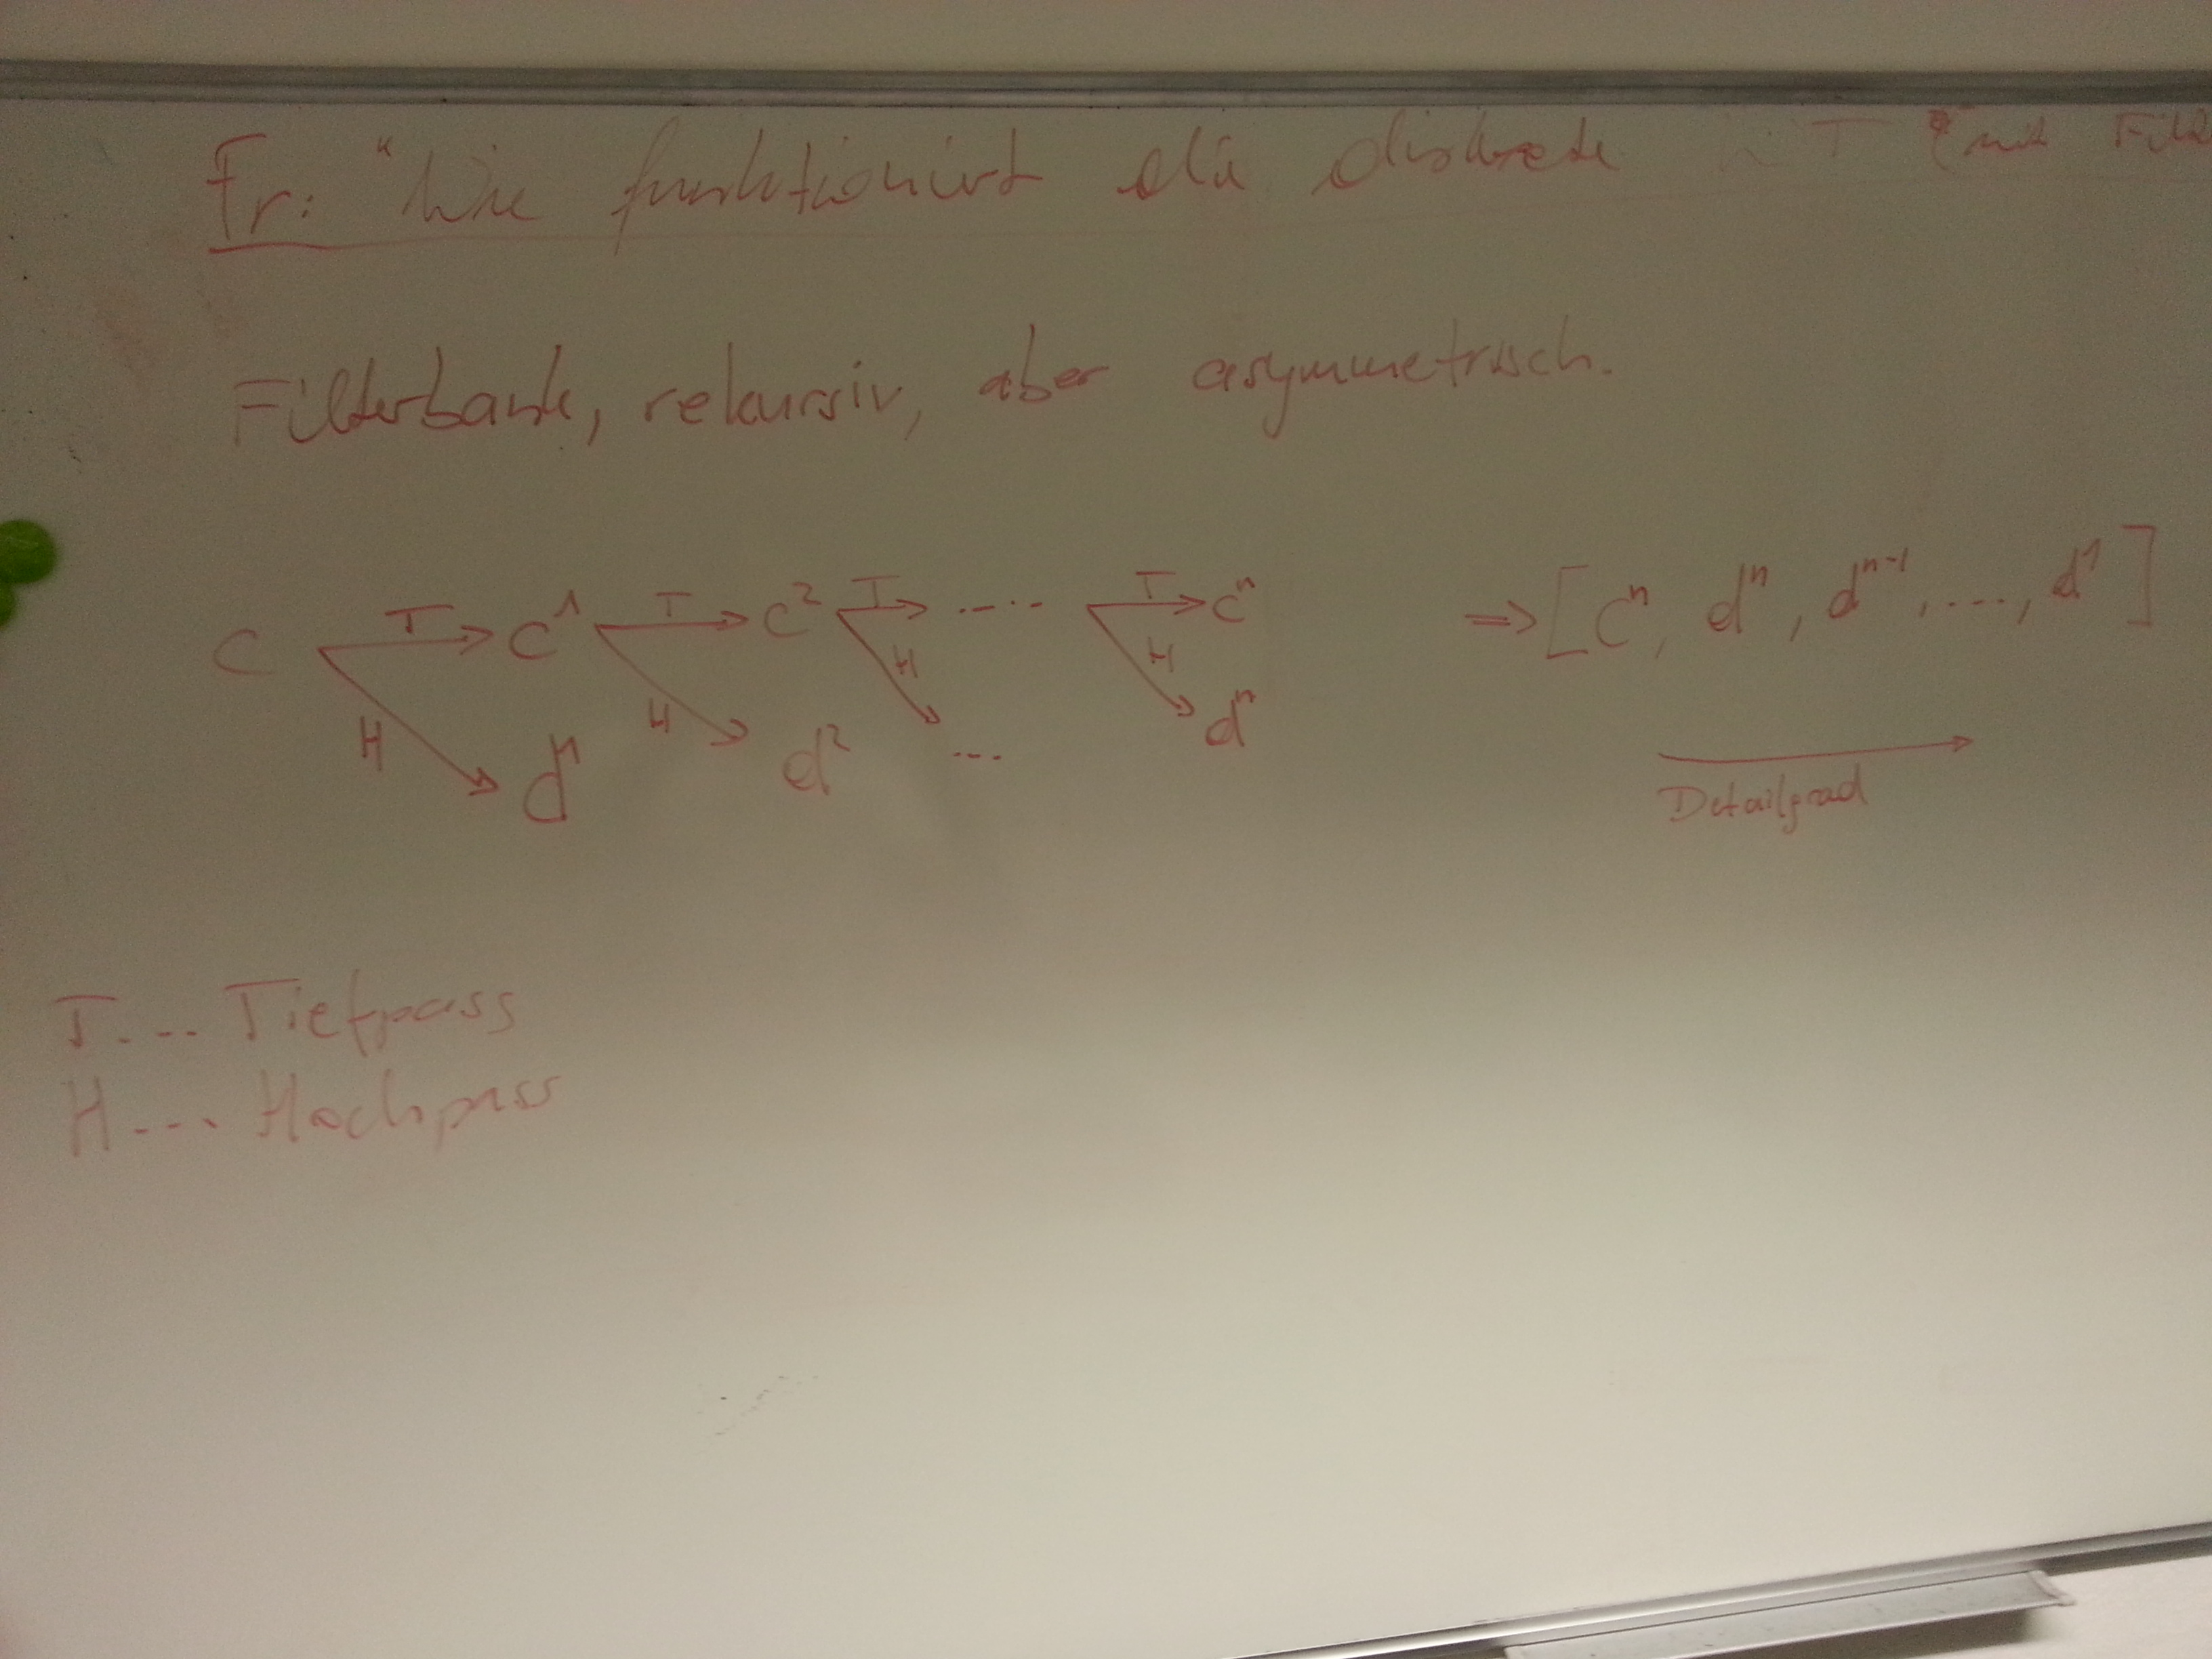
\includegraphics[width=\linewidth]{Fotos/Filterbank1}
    \caption{Skizze einer Filterbank.}
    \label{fig:Filterbank1}
    \end{figure}
	\item[Nenne 3 typische Filter]
  	Binomialfilter (Glättung), Medianfilter (Glättung), Laplace-Filter (Kantendetektion).
	\item[Was ist die zentrale Eigenschaft von Filterbänken? Welche Voraussetzung muss dazu gelten?]
  	Man startet mit einen Signal $ c $, generiert daraus den Polyphase-Vektor $ P $, stecke diesen 
  	in die Analyse-Filterbank. Das Ergebnis davon kommt in die Synthese-Filterbank, daraus bekomme 
  	ich einen weiteren Polyphase-Vektor, den ich dann ein Ausgangssignal $ c' $ umwandeln kann.
  	Der Polyphase-Vektor ist sozusagen eine vektorwertige Abtastung des Signals auf dem 
  	Einheitsmatrix. Die Modulationsmatrix $ M $ ist eine darstellende Matrix der 
  	Analyse-Filterbank, und $ \widetilde{M} $ die darstellende Matrix der Synthese-Filterbank.
  	Soll Perfect Reconstruction gelten, d.h.\ dass $ c = c' $ gilt, dann muss ich alle Änderungen, 
  	die $ M $ gemacht hat, auch wieder rückgängig machen können durch $ \widetilde{M} $. 
  	Mathematisch: $ M \widetilde{M} = I $. Voraussetzungen an die Filter in der Filterbank werden 
  	bereits durch die Modulationsmatrizen $ M $ und $ \widetilde{M} $ gegeben.
  	
  	Mathematische Formeln:
  	\begin{itemize}
    	\item Polyphase-Vektor
    	\[
      	P = \left( c^{*}(e^{2i\pi k/n}z) \colon k \in \Z_{n} \right) \in \C^{n}.
    	\]
    	\item Darstellende Matrix
    	\[
      	M(z) =
      	\frac{1}{n} \left( f^{*}_{j}(e^{2\pi i k / n}) \colon j,k \in \Z_{n} \right) 
      	= \frac{1}{n} \begin{pmatrix}
      	f^{*}_{0}(z) & \hdots
      	\end{pmatrix} \in \C^{n \times n}.
    	\]
    	Dabei ist $ f_{j} $ jeweils die Impulsantwort eines Filters $ F_{j} $
  	\end{itemize}
	\item[Kann man Filterbänke hierarchisch aufbauen?]
  	Natürlich kann man das! Dieses Ding nennt man dann Subband-Coding. Beispiel: $ n = 2 $. Dann 
  	starte ich mit meinem Signal, filtere das mit einem Tiefpassfilter $ F_{0} $ und Hochpassfilter 
  	$ F_{1} $. Dann mache ich ein Downsampling um den Faktor $ 2 $. Dies liefert mir im Falle des 
  	Tiefpassfilters ein Singal $ c_{0} $. Dieses Signal kann ich nun auf die gleiche Art und Weise 
  	wieder rekursiv zerlegen. Dabei verwende ich wieder den Filter $ F_{0} $ (Tiefpass) und ein 
  	Downsampling um Faktor $ 2 $, um ein Singal $ c_{00} $ zu bekommen. Analog erhalte ich $ c_{01} 
  	$ durch den Hochpassfilter. Das war die Analysephase.
  	
  	In der Synthesephase nehme ich meine Signale $ c_{00} $ und $ c_{01} $, wende den 
  	Upsampling-Operator um Faktor $ 2 $ an, wende dann die Filter $ G_{0} $ und $ G_{1} $ an, fasse 
  	die beiden Ergebnisse zu einem Signal $ c_{0} $ zusammen. Und mit $ c_{0} $ und $ c_{1} $ kann 
  	ich dann das gleiche wieder rekursiv machen. Zum Schluss erhalte ich das Signal $ c $, welches 
  	mit dem ursprünglichen Eingabesignal übereinstimmen kann, aber nicht muss.
  	Signal 
  \item [Wie funktioniert die Diskrete Wavelet-Transformation mit Filterbänken?] 
    $ \rightarrow $ siehe Abbildungen~\ref{fig:Filterbank2} und~\ref{fig:Filterbank3}.
    \begin{figure}[ht]
    \centering
    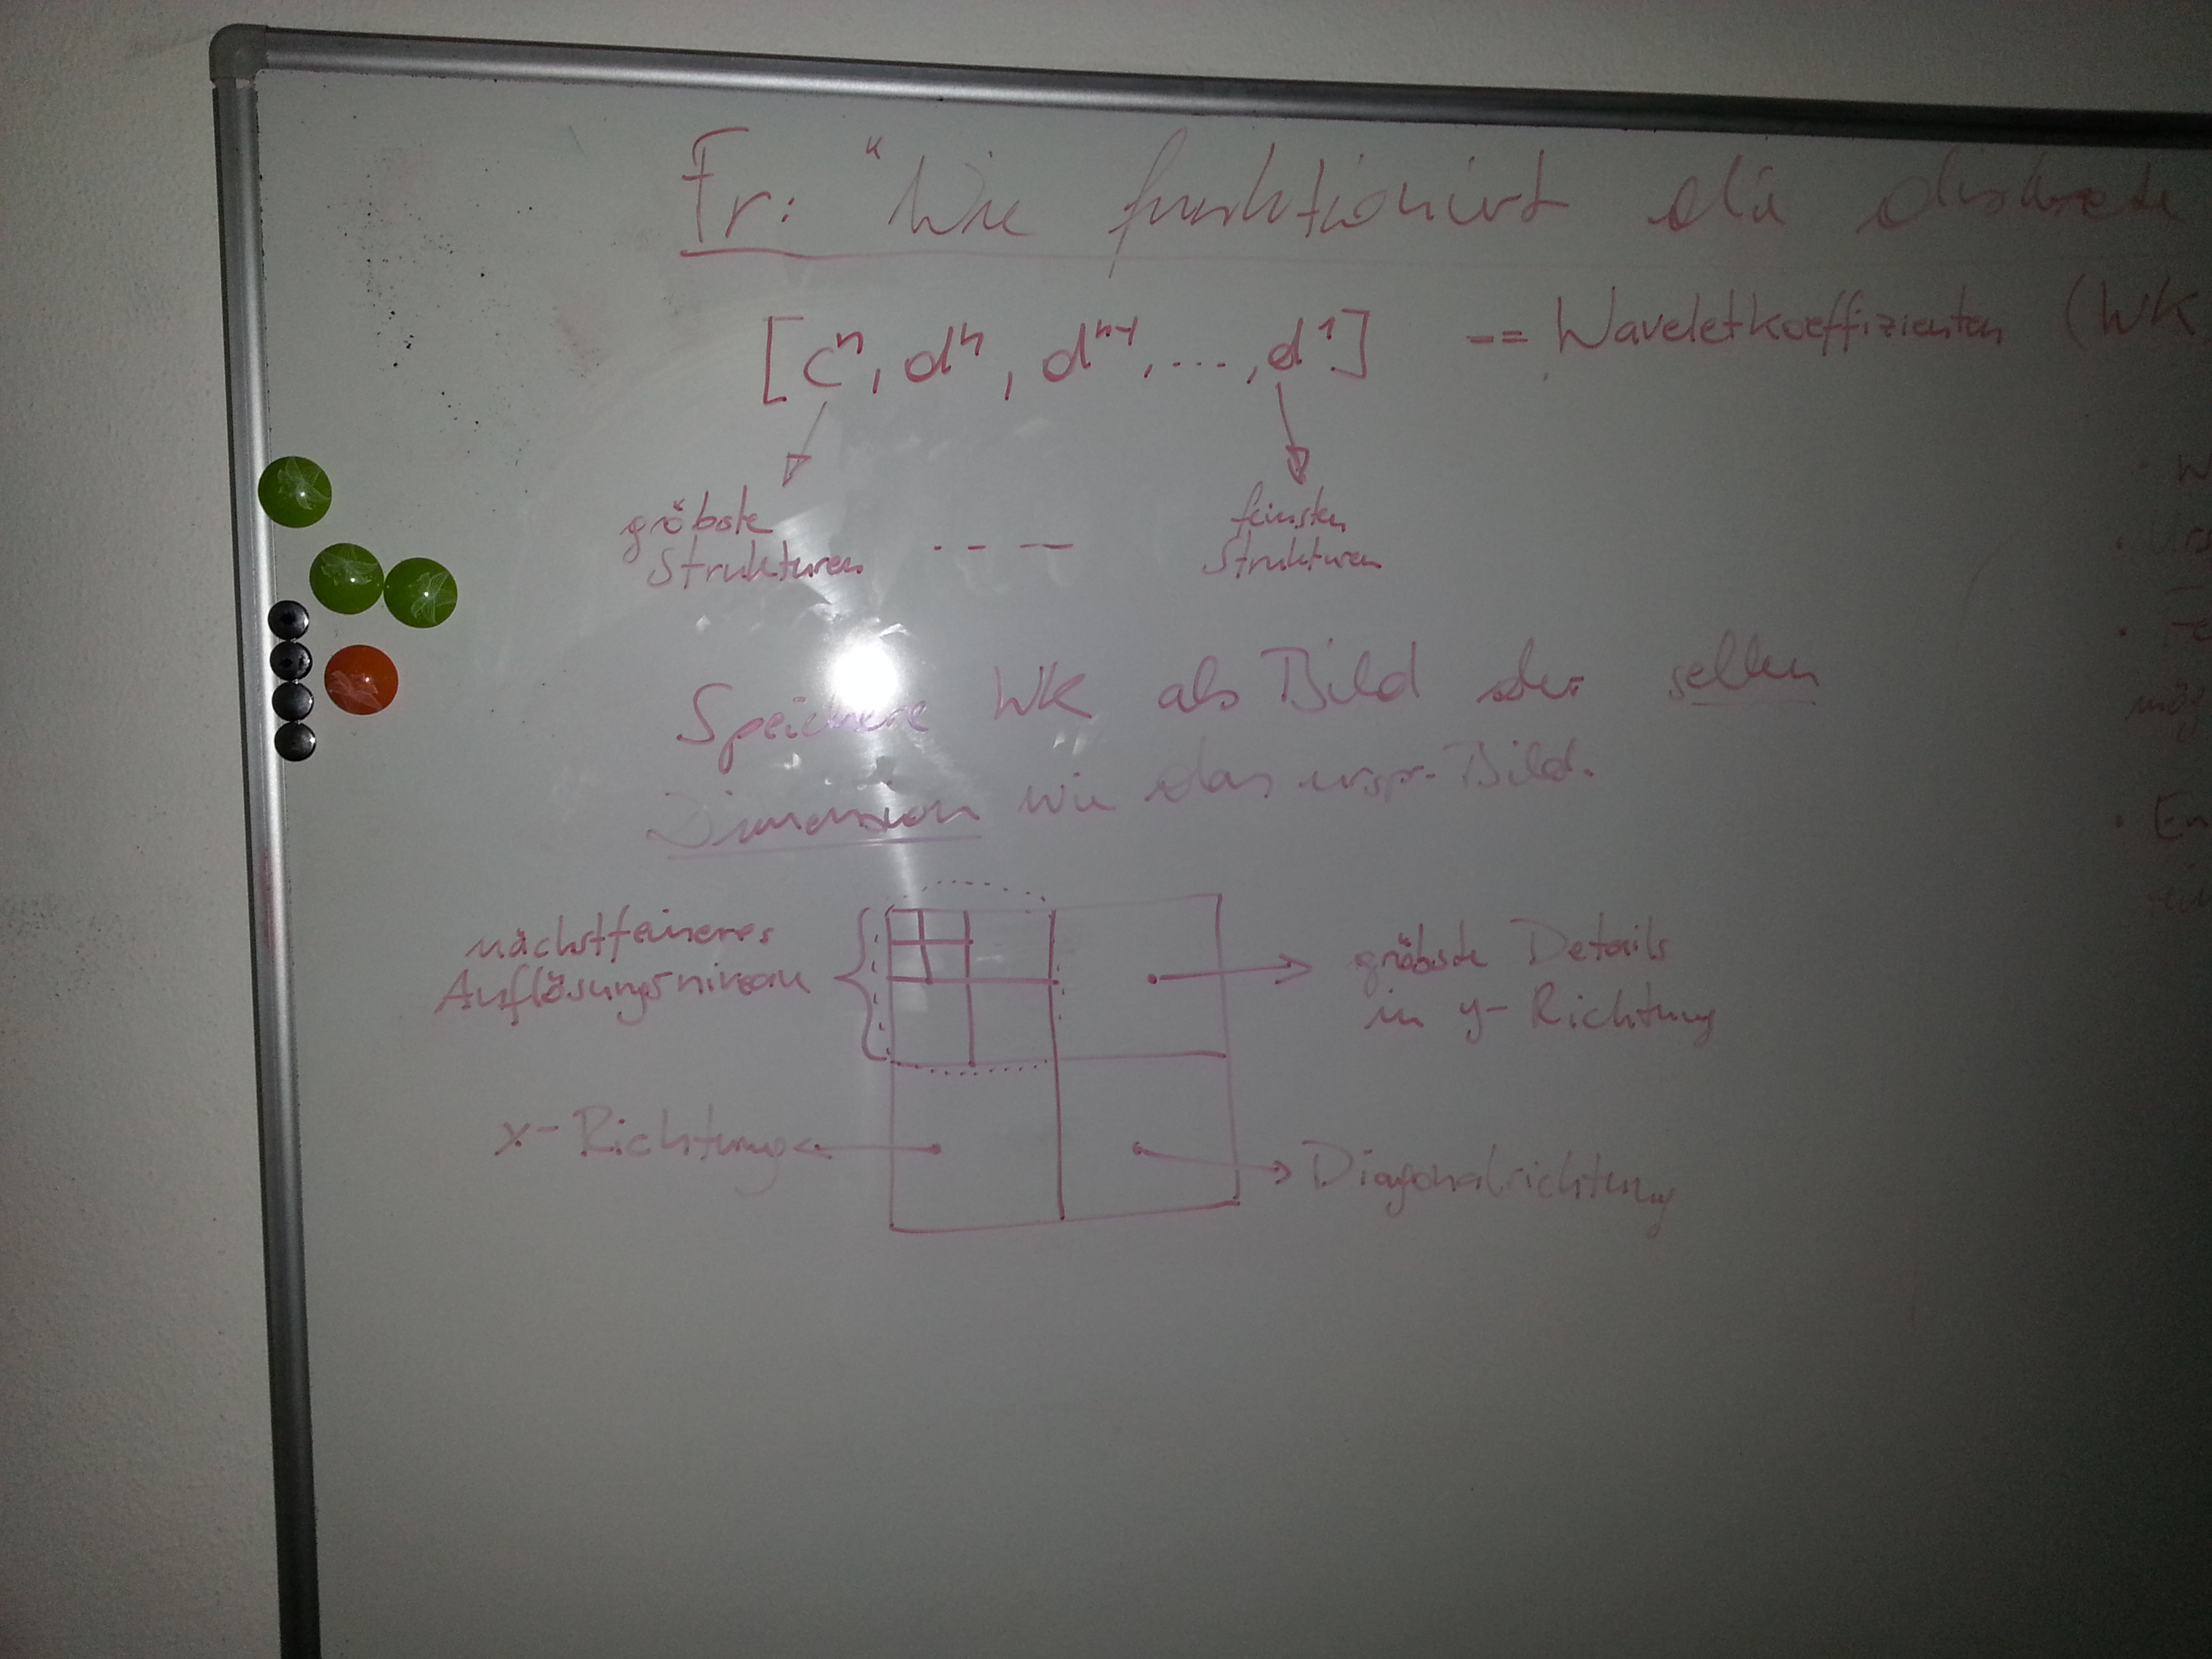
\includegraphics[width=\linewidth]{Fotos/Filterbank2}
    \caption{}
    \label{fig:Filterbank2}
    \end{figure}
    \begin{figure}[ht]
    \centering
    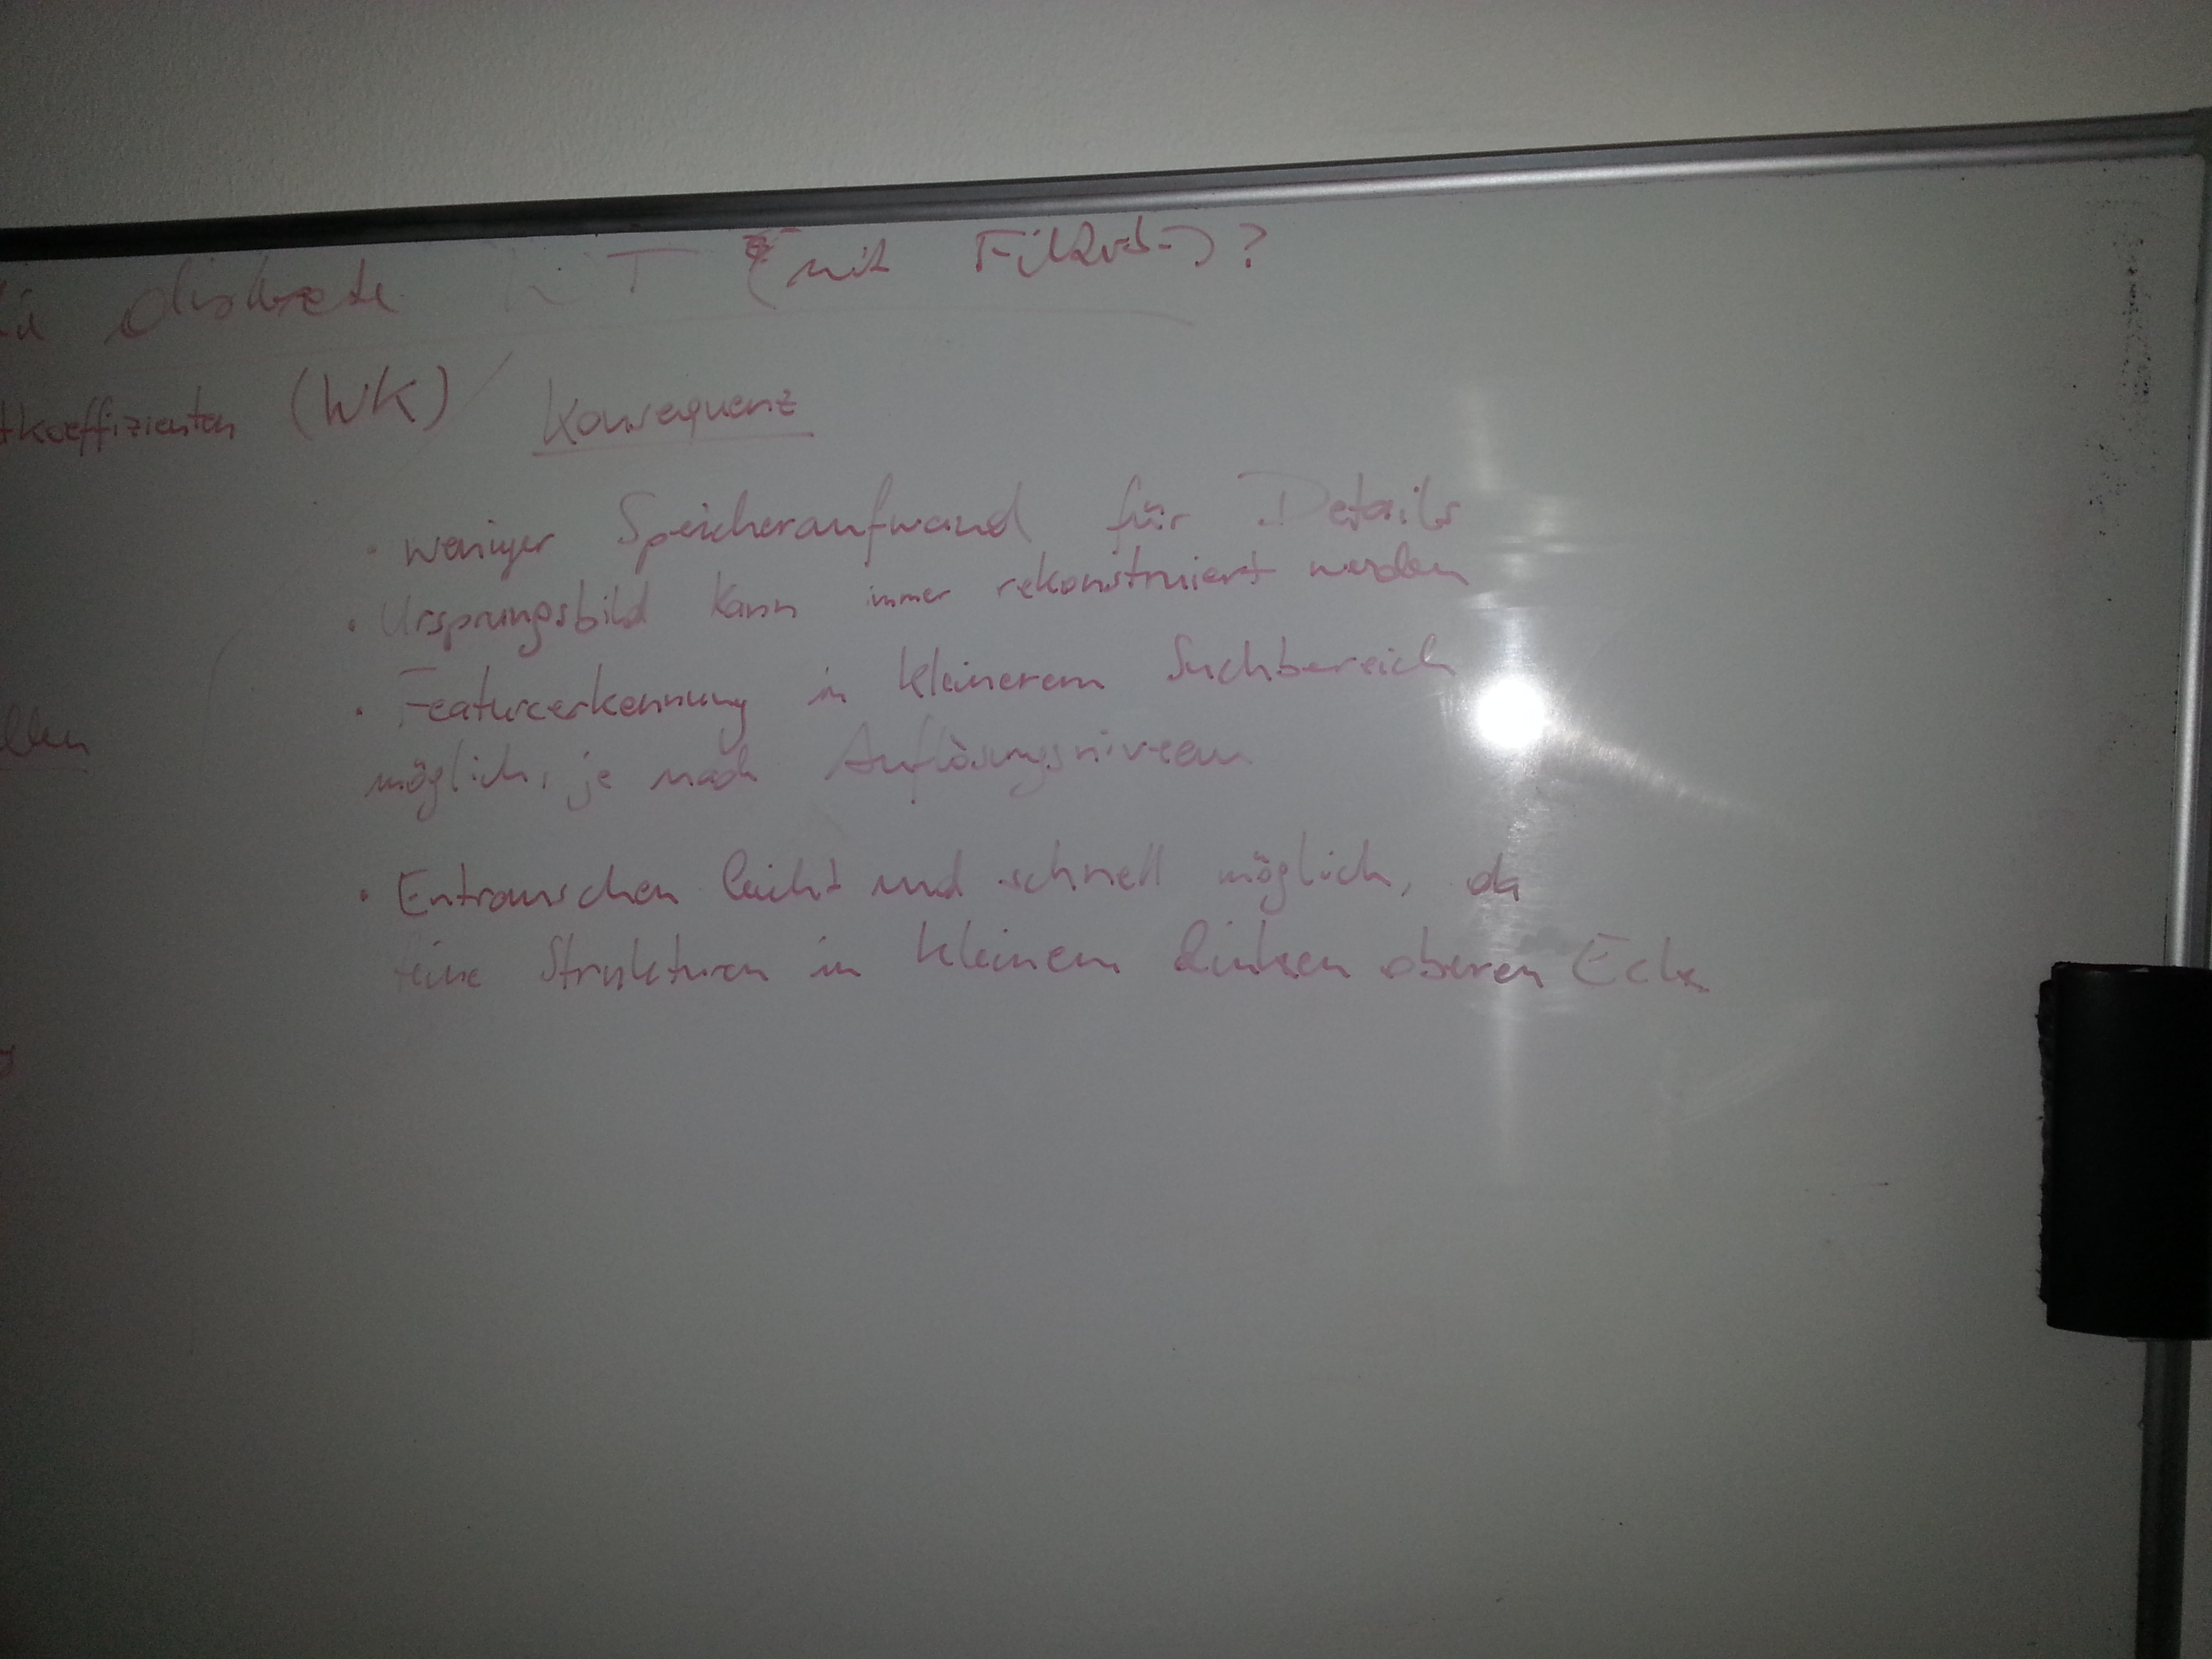
\includegraphics[width=\linewidth]{Fotos/Filterbank3}
    \caption{}
    \label{fig:Filterbank3}
    \end{figure}
\end{description}
\section{Abtastsatz}
\begin{description}
	\item[Welche Eigenschaften müssen für eine Abtastung gelten?]
  	Funktion muss integrierbar sein. Schrittweite der Abtastung muss kleiner sein als $ h^{*} $, um 
  	Unterabtastung zu vermeiden, und die Funktion muss bandbeschränkt sein, weil man nicht 
  	unendlich viele Frequenzen rekonstruieren kann.
	\item[Erkläre den Shannonschen Abtastsatz]
      Der Shannon'sche Abtastsatz sagt, dass wenn man eine $T$-bandbeschränkte $L_1$-Funktion fein genug
      abtastet, dann kann man aus dieser Abtastung durch eine semi-diskrete Faltung mit der \emph{sinc}-Funktion
      die Originalfunktion eindeutig rekonstruieren.
	\item[Wie funktioniert Abtasten überhaupt?]
      Beim Abtasten mit Faktor $h$ nimmt man nur jeden $h$-ten Funktionswert in die Evaluation auf.
      Formal nimmt man also nur jeden $c(h\cdot)$-ten Wert auf.
	\item[Was ist die kritische Abtastrate?]
      Die kritische Abtastschrittweite ist der Kehrwert der sogenannten Nyquist-Frequenz. Das bedeutet, dass
      man mit einer höheren Frequenz als der Nyquist-Frequenz (und damit mit einer kleineren Abtastschrittweite) 
      abtasten muss, um die Funktion (sofern überhaupt möglich) eindeutig aus der Abtastung rekonstruieren zu können.\\
      Tastet man zu grob ab, so kommt es zu \emph{Überlagerungen}, wo man im Nachhinein nicht mehr sagen kann, zu welchem
      Teil des Signals welcher Teil der Überlagerung gehört.
	\item[Wie berechnet man die kritische Abtastrate?]
      Die Nyquist-Frequenz einer $T$-bandbeschränkten Funktion ist gegeben durch $T/\pi$, entsprechend ergibt sich
      die kritische Abtastschrittweite durch deren Kehrwert, also $h^* = \pi/T$.\\
      Um nun die angesprochene eindeutige Rekonstruktion zu bewerkstelligen, muss man mit einer Schrittweite von
      $h < h^*$ abtasten.
	\item[Was ist ein bandbeschränktes Signal?]
      Ein bandbeschränktes Signal $f\in L_1(\R)$ ist ein Signal, welches nur ein \emph{beschränktes Band} and Frequenzen
      ($[-N,N], N\in\R$) beinhaltet\footnote{Was ja auch durchaus realitätsnah ist.}, formal:
      $$ \hat f(\xi) = 0 \Leftrightarrow \xi \not\in [-N,N]\quad,\xi\in\R $$
	\item[Was ist der Träger eines Signals?]
      Der Träger eines Signals ist umgangssprachlich definiert als der Bereich auf der Zeitachse, auf der
      das Signal \emph{lebt}. Formal ist der Träger
      $$ \text{supp} f = \{t \in \R \colon f(t) \neq 0 \} \subset \R $$

      In einem realen Anwendungsfall wir ein Signal immer endlichen Träger $[a,b]\subset\R$ haben, 
      also gilt für ein passendes Maß $\INTM{\mu}$, dass $\INTM{\mu}([a,b]) < \infty$ ist.
\end{description}
\section{Transformationen}
\subsection{Hough-Transformation}
\begin{description}
	\item[Was ist die Hough-Transformation?]
      % Ja, hier hab ich textbf verwendet, weil ich das explizit fett haben will, nur so zur Info ...
      Die Hough-Transformation ist ein allgemeines Verfahren, um in einem \textbf{binearisierten} Bild Formen zu erkennen.
	\item[Wie funktioniert sie?]
      Bei der Hough-Transformation wird für alle möglichen Variationen einer Form im gesamten Bild
      gesucht, ob diese vorkommt. Dies wir dadurch realisiert, dass man bei der Test-Form alle Pixel gezählt
      werden, bei der in der binearisierten Form ein Farbwert (z.B. 1 für Schwarz) steht. Hat man nun eine hohe Anzahl
      gefunden, so hat man ziemlich sicher auch die gesuchte Form im Bild erkannt.
	\item[Was ermöglicht sie?]
      Mit diesem Verfahren kann man nun nach \emph{allen möglichen} Formen in Bildern suchen, die Formen müssen sich 
      entsprechen parameterisieren lassen. Dies ist u.a. für Linien, Kreise, Ellipsen u.v.m. möglich.

      Man beachte aber, dass man z.B. bei Linien zwei Freiheitsgrade hat. D.h. man muss für alle Möglichkeiten dieser
      Freiheitsgrade das Bild absuchen, was hier schon quadratischen Aufwand liefert. Will man nun z.B. Kreise finden,
      so hat man schon drei Freiheitsgrade (die $x$- und die $y$-Koordinate des Mittelpunktes und den Radius $r$), was
      entsprechend kubischen Aufwand liefert.
    \item[Was sind mögliche Optimierungsmöglichkeiten?]
      Mögliche einfache Optimierungen sind z.B., dass man die Freiheitsgrade einschränkt. Sucht man z.B. in einem Bild
      nur nach Kreisen mit einem festen Radius, so besteht die einzige Variationsmöglichkeit in den Koordinaten des
      Kreismittelpunktes, was insgesamt also quadratischen Aufwand verursacht.
	\item[Welcher Filter spielt dabei eine Rolle?]
  	Man muss das Bild vorher z.B.\ durch einen entsprechenden Filter binarisieren.
	\item[Gibt es weitere Filter zur Kantenerkennung?]
      Der wohl einfachste (und schnellste) Filter zur Kantenerkennung ist ein Bildshift. Damit shiftet man das Bild
      in die Richtung, in der man Kanten finden möchte um eine Position. Ist der Unterschied hoch, so unterscheiden
      sich die Farbwerte signifikant, also liegt vmtl eine Kante vor.\\

      Eine andere Möglichkeit ist die Betrachtung eines Differenzbildes.\\

      Eine nette Alternative, die sich massivst parallelisieren lässt, ist der Sobel-Operator. Dieser Filter nimmt die
      Farbwerte benachbarter Pixel gewichtet und errechnet daraus einen neuen Wert\footnote{Stencil und so.} und findet
      so Kanten.\\

      Eine weitere, jedoch ziemlich unbrauchbare Möglichkeit ist die Verwendung der Fouriertransformation. Dabei erhält
      man zwar die Information, dass es Kanten im Bild gibt, aber nicht wo, da man keine Lokalitätsinformationen 
      hat\footnote{Das ist ein Statement vom Matheman, das ich für ziemlich unbrauchbar halte, aber der Vollständigkeit
      halber sei es hier erwähnt.}.\\

      Eine weitere, moderne Alternative ist die Verwendung von Wavelets. Damit erkennt man Kanten durch die schnellen
      Änderungen von Frequenzen. Zusätzlich weiß man auch, wo sich diese Kanten befinden, da man bei der Wavelettransformation
      ja Lokalitätsinformationen hat.
\end{description}
\subsection{Gabor-Transformation}
\begin{description}
  \item[Was ist die Gabor-Transformation?]
    Die Gabor-Transformation ist eine \emph{gefensterte} Fouriertransformation.\\
    Formal gilt also für $f,g \in L_2(\R), g \text{ gerade und }\|g\|_2 = 1$:
    $$ Gf(u,\xi) = \int_\R f(t) e^{-i\xi t} g(t-u) \INT{t} $$
  \item[Was ist ein Spektrogramm?]
    Ein Spektrogramm ist ein Diagramm, auf denn $x$-Achse die Zeit und auf der $y$-Achse die Frequenz aufgetragen ist.
    Das spiegelt also wider, wieviel Energie sich zu einer Zeit in einer gewissen Frequenz konzentriert.
  \item[Wie hängt die Gabor-Transformation mit der Fouriertransformation zusammen?]
    Durch die Fensterfunktion bekommt man eine gewisse Lokalitätseigenschaft, da man dann Aussagen über die
    Frequenzanteile in dem spezifizierten Zeitfenster treffen kann, während sich die reine Fouriertransformation diese
    Informationen global ansieht.
\end{description}
\subsection{Wavelets}
\begin{description}
  \item[Was ist ein Wavelet?]
    Ein Wavelet $\Psi$ ist eine beliebige $L_2$-Funktion, die die Eigenschaft der Mittelwertfreiheit erfüllt, also dass gilt
    $$ \int_\R \Psi(t) \INT{t} = 0. $$ Der Name kommt daher, dass diese Funktionen wie Wellen aussehen müssen (also Anteile
    über und unter der $x$-Achse), um in der Fläche $0$ zu sein.
  \item[Was bedeutet Zulässigkeit bei Wavelets?]
    Die Zulässigkeit bei Wavelets ist eine mathematische Bedingung, dass 
    $$ C_\Psi := \int_\R \frac{\left|\hat \Psi(\xi)\right|^2}{|\xi|}\INTM{\xi} < \infty $$
    gelten muss. Um dies zu gewährleisten sollte die Funktion an der $0$ insbesondere $0$ sein, 
    weil man selten gut durch Null dividieren kann.
    
    Die Zulässigkeit ist insbesondere eine Voraussetzung dafür, dass man die Inverse Wavelet-
    Transformation berechnen kann, weil sonst der Term $ \frac{1}{C_{\psi}} $ null wäre und dann
    würde man als Rekonstruktion die konstante Nullfunktion erhalten.
  \item[Was ist die Wavelet-Transformation?]
    Die Wavelet-Transformation ist eine integraltransformation, welche das Signal und das Wavelet quasi als Fensterfunktion
    miteinander in Beziehung setzt:
    $$ \mathcal{W}_\Psi f(u,s) := \int_\R f(t) \frac{1}{\sqrt{|s|}}\overline{\Psi\left(\frac{t-u}{s}\right)}\INT{t} $$
  \item[Was ist ein Skalogramm?]
    Ein Skalogramm ist das Analogon zum Sprektrogramm der Gabor-Transformation, mit dem Unterschied, dass nun auf der
    vertikalen Achse nicht die Frequenzen sondern die \emph{Skalen} aufgetragen sind, was in etwa dem Kehrwert der 
    Frequenzen entspricht. Die (Farb-)Werte im Diagramm selbst wird dann die Intensität da sein.
  \item[Was sind Heisenberg-Boxen?]
    Die Heisenberg-Boxen sind die graphischen Elemente des Skalogramms. Diese werden durch insgesamt vier Parameter 
    definiert:

    \begin{enumerate}
      \item Zeitauflösung $\mu$
      \item Frequenzauflösung $\hat \mu$
      \item Zeitvarianz $\sigma$
      \item Frequenzvarianz $\hat \sigma$
    \end{enumerate}

    Die Zeit- und die Frequenzauflösung bilden zusammen den Mittelpunkt der Box im Diagramm, während die Varianzen
    die halbe Ausdehnung der Boxen in die jeweiligen Achenrichtungen darstellen.

    Graphisch (oder semi-graphisch) dargestellt:

    \begin{lstlisting}
      +----------------------------------------+
      |                                        |
      |                                        |
      |                   x (mu, hat mu)       |<---|
      |                                        |    | \hat sigma
      |                                        |    |
      +----------------------------------------+<---|
                          ^                    ^
                          |____________________|
                                   sigma
    \end{lstlisting}
  \item[Was besagt die Heisenberg'sche Unschärferelation?]
    Die Heisenberg'sche Unschärferelation besagt, dass diese Heisenberg-Boxe eine Mindestfläche
    besitzen. Das bedeutet insbesondere, dass man nicht beliebig genau in Zeit und Frequenz auflösen
    kann. Dies ist aber auch der Natur nachempfunden, da z.B. ein Ton mit einer niedrigen Frequenz
    relativ lange schwingen muss, um gehört zu werden.
  \item[Warum findet sich bei vielen Wavelets der Gauß-Kern als Term wieder?]
    Dies liegt daran, dass man mit dem reinen Gauß-Kern prinzipiell die bestmögliche Zeit-/Frequenz-
    Auflösung bekommen würde (also hat die Heisenberg-Box dann minimale Fläche). Das Problem ist nur,
    dass der Gaußkern kein Wavelet ist, da nicht mittelwertfrei.
  \item[Was ist der Vorteil der Wavelet-Transformation gegenüber der Fourier- bzw Gabor-Transformation?]
    Der klare Vorteil hierbei liegt darin, dass sich die Heisenberg-Boxen (und damit die Auflösung)
    dynamisch an die Frequenz oder Zeit anpasst. Bei Gabor legt man durch die Fensterfunktion aber eine
    fixe Frequenz-/Zeit-Auflösung fest. Man bekommt mit der Wavelet-Transformation also eine dynamische
    Zeit-/Frequenz-Auflösung mit einer gewissen Lokalitätseigenschaft.
    Bei der Wavelet-Transformation gilt: Je \enquote{unglatter} die Funktion ist, desto höher ist
    die Abklingrate der Wavelet-Koeffizienten.
  \item[Wo spiegelt sich bei der Wavelet-Transformation Redundanz wider?]
    Man kann\footnote{Man kann, ich kann es nicht ...} mathematisch nachweisen, dass man die Originalfunktion
    aus der Wavelet-Transformation mit nur einer einzigen Skala rekonstruieren kann.
  \item[Gibt es praktische Anwendungen für die Wavelets?]
    Ein prominentes Beispiel\footnote{Ein prominentes Beispiel, was dennoch kein Schwein hernimmt (facepalm).}
    ist z.B. Bildkompression mit JPEG-2000.
\end{description}


\end{document}